\documentclass[thesis.tex]{subfiles}
\begin{document}

\chapter{Introduction}
\label{chap:introduction}

% An image right here at the top can look really cool!

\section{Introduction}
The current Internet has exceeded any expectations in terms of reach or various applications. The engineers creating it in the 1960s couldn't even imagine the impact on the society and various use of their creation. Only few users who know each other participated in the early Internet without considering security and protection against attacks as a key aspect.

Today 50 years later there are billions of users and devices connected to each other \cite{MiniwattsMarketingGroup.31.12.2017}, using different application from e-mail, streaming of video and audio or chatting which each other. Unfortunately, there are also malicious users trying to disturb the network by overusing resources or manipulating data to deceive the members. More and more services are created each year running on the Internet and trying to provide a service to users. Each company has to know the newest security risks and attack types to be competitive and trustworthy. 

This growing interest and their security is only covered by multiple patches and fixes for the Internet Protocols. The problem of such an approach is that it must be first accepted by the majority of the users and then supported by network device manufacturers and administrators. For example, the acceptance of IPv6, a protocol released in 1996, is low in 2017 but the Internet ran out of IPv4 addresses in 2011 \cite{ICANN.03.02.2011}.

Instead of fixing the current Internet and trying to patch the structural problems from past designs, there are also people creating a new solution. They want to solve the problems without limitations of the current protocols and their implicit fundamental problems. One of the solutions is \textbf{SCION}\cite{SCIONBook, SCIONPaper}, that stands for \textbf{S}calability, \textbf{C}ontrol and \textbf{I}solation \textbf{O}n next-generation \textbf{N}etworks, which will be explained in detail in \autoref{chap:preqAndRel}.

\section{Motivation}
One of the many issues is the strong increase of traffic on the Internet. The DE-CIX in Frankfurt, Germany, a data carrier, accounts each year a higher amount of data as shown in \autoref{fig:intro:decixData}. In 2014 the peak was around three TB/s. Three years later in 2017 the peak was at 6 TB/s, i.e. twice the amount. 

In the advent of video streaming in form of Video on Demand (VOD) via services like YouTube\footnote{\url{https://www.youtube.com}, 20.04.2018} and Netflix\footnote{\url{https://www.netflix.com}, 20.04.2018} and live video streaming like Twitch\footnote{\url{https://www.twitch.tv/}, 20.04.2018} the data usage of the users increased rapidly. There is also an increasing demand for higher resolutions, which results in bigger video sizes. The current standard of Full HD for a video will be succeeded by new standards like the 4K. The user also demands for a higher frame rate. Currently, the videos are sent with 30fps, but there is a benefit using 60fps or even 144fps for really fast movements.

But videos are not the only reason for a higher bandwidth usage. Big Data companies processing petabytes of data each day rely on a stable and high bandwidth connection. There is also a trend with Internet-of-Things (IoT) to install small devices which collect and send data through the Internet.

The poor stability of the current Internet is also a motivation to improve the structure of it. Attacks like \textbf{D}istributed \textbf{D}enial-\textbf{o}f-\textbf{S}ervice (DDos) using the resources to disrupt the operation of companies or governments are increasing in size and frequency \cite{GoogleInc.2013}. But also technical problems like a power outage \cite{DECIX.10.04.2018} or an environmental hazard (earthquakes, floods) can disturb the stability of the Internet when a central node fails. 

\begin{figure}
    \centering
    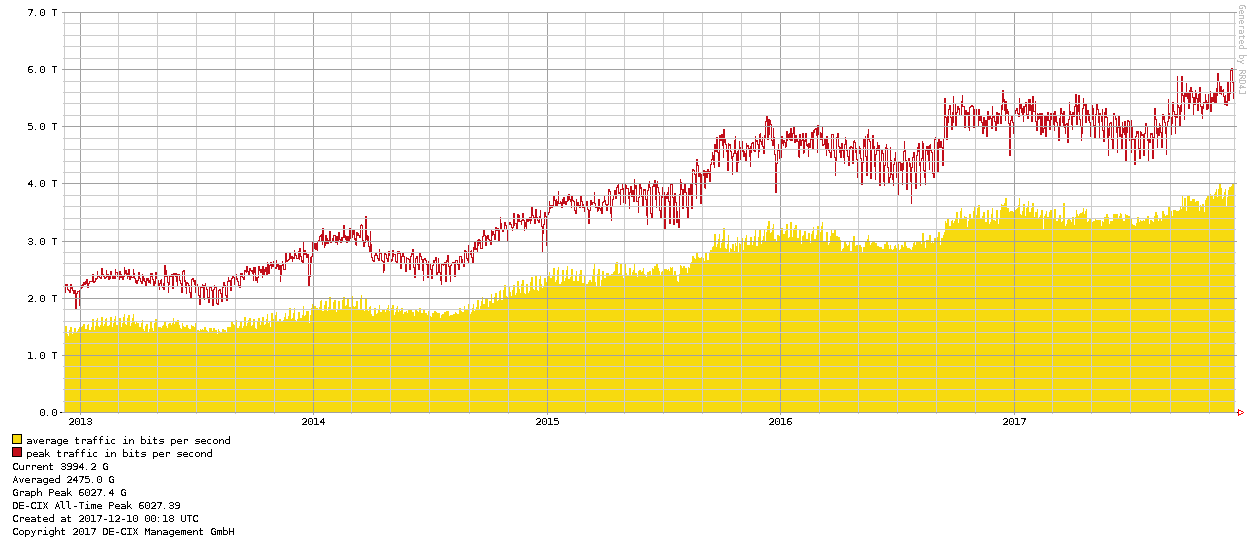
\includegraphics[width=0.95\linewidth]{20171210_1515_decix_data}
    \caption*{\tiny{ \url{https://www.de-cix.net/en/locations/germany/frankfurt/statistics} (10.12.2017)}}
    \caption{5-year graph of the average exchanged traffic at DE-CIX in Frankfurt, Germany}
    \label{fig:intro:decixData}
\end{figure}

One solution to solve these problems is to scale-up and install more and more bandwidth capacities like fiber cables or newer devices. This is inefficient and consumes probably more energy and thus increases the running costs. There are also physical limitations for improving the performance so that a small benefit results in high costs.

Another solution is to better utilize the current resources as it is done with the multi-path feature in SCION. It allows the users to split their data and send the packets via multiple connections. This leads to a better usage of the available bandwidth in the network. In the current Internet this is not possible, because the routers are deciding for themselves which route to take to the destination. 

\begin{figure}[h]
    \centering
    \begin{tikzpicture}
    \node[shape=rectangle,draw=black] (1-1) at (0,0) {1-1};
    \node[shape=rectangle,draw=black] (1-2) at (2,-1) {1-2};
    \node[shape=rectangle,draw=black] (1-3) at (2,1) {1-3};
    \node[shape=rectangle,draw=black] (1-4) at (4,0) {1-4};
    
    \path[-]	
    (1-1) edge node[sloped, anchor=center, below] {\tiny 1GB/s} (1-2) 
    (1-1) edge node[sloped, anchor=center, above] {\tiny 1GB/s} (1-3)
    (1-1) edge node[sloped, anchor=center, above] {\tiny 1GB/s} (1-4)
    (1-2) edge node[sloped, anchor=center, below] {\tiny 1GB/s} (1-4)
    (1-3) edge node[sloped, anchor=center, above] {\tiny 1GB/s} (1-4)
    ;
    \path[-{Latex[width=3mm]}, dashed]
    (1-1) edge[bend right=10] (1-4)
    (1-1) edge[bend left=80] (1-4)
    (1-1) edge[bend right=80] (1-4)
    ;
    \end{tikzpicture}
    \caption{Example topology for multi-path communication.}
    \label{fig:intro:exampleMultipath}
\end{figure}

This new method shall encourage users to better utilize the network, but it can also be misused. In \autoref{fig:intro:exampleMultipath} an example is visualized. Each node represents an \textbf{A}utonomous \textbf{S}ystem (\textit{AS}). All ASes in this figure but not 1-2 to 1-3 are connected with each other via a 1 GBit/s connection. AS 1-1 can send AS 1-4 data using single path with a 1 GBit/s directly. It could also use the paths 1-1$\rightarrow$1-2$\rightarrow$1-4 and 1-1$\rightarrow$1-3$\rightarrow$1-4 to send its data and increase its bandwidth to ideally 3 gigabit/s, if there is zero delay on the hops. This possibility rises the questions how to monitor and enforce the bandwidth usage of one particular AS. When using a single path connection the measurement point is at the destination. If this AS exceeds its limit the destination router can drop packets. This solution is not possible in a multi-path environment, because a single destination router is missing the information about the cumulative bandwidth of the source node. It is important to find an answer for this question to avoid misuse.

\section{Goals} \label{sec:intro:goals}

The work was planned and executed with the following described goals in mind. They will be evaluated in \autoref{chap:eva} and tested if they have been achieved by the proposed approach in this work.
     \begin{easylist}
        \MyNumberedListProperties
        # The thesis' main goal is to propose a mechanism to identify network users who overuse their resources in a multi-path environment. These are considered \textit{greedy}.
        # It is a goal that the solution must achieve a trade-off between the accuracy and the mechanism's efficiency. A detection rate of 100\% is not necessary when the cost of computation time and memory is too high to be realizable on a network component. 
        # There must be parameters to configure the detection mechanism. A network administrator can increase the detection rate when the additional performance impact is acceptable or the other way around. This results in a better acceptance of the solution.
        # The solution must be general enough to be adapted for other network types supporting multi-path communication. The solution can define requirements outside the multi-path capability to be working in such a network type.
        # Scalability is important for networks because of their growing size. The proposed answer must be able to scale with the size of the network in terms of detection rate and performance impact. 
        # Based on the previous goals, the work will contain an implementation for SCION which can be used in its testbed SCIONLab. It is not a goal to provide a production ready application but a working prototype which scales and detect malicious users.
    \end{easylist}

\section{Main Contribution}
The proposed contribution will provide a solution to identify greedy users inside a network with a small impact on the networks' performance. It will use a heuristic based selection algorithm to only monitor interesting nodes. This leads to a small amount of necessary nodes to receive a high enough coverage of the networks traffic to identify nodes which overuse their resources. The approach will be created for networks in general and will have a proof of work implementation for the SCIONLab network structure.

\section{Thesis Outline}
This thesis is divided into five chapters and an appendix. The first chapter \autoref{chap:introduction} introduced the problem and provided a motivation for solving this problem. It defined goals to get achieved and outlined the main contribution to the topic.

The next chapter \autoref{chap:preqAndRel} explains the necessary requirements to be able to understand and follow this work and related work to this topic. It explains how the SCION network functions and what the used tool for this work is. The related work section will contain already existing works similar to the topic, such as SIPRA for SCION itself and results of other researchers. 

The third chapter, \autoref{chap:main} describes the main contribution of this work, the SpeedCam approach based on the inspection game. It is first described in a concept for networks in general and then specialized for the SCION structure. This chapter will also formulate theses and assumptions of the influence of featured variables.

These will be evaluated in \autoref{chap:eva}, which contains the experiment to show the results. Firstly it will describe the setup for the evaluation and will then show and discuss the results of it.

This work will be concluded in the last chapter \autoref{chap:concl}. This will summarize the work, show the implications of the results and give an overview of new questions and problems to solve in further works.

The appendix will contain configurations and listings to reproduce the results.

\subfilebib % Makes bibliography available when compiling as subfile
\end{document}